%:
% !TEX TS-program = pdflatex
% !TEX encoding = UTF-8 Unicode

% This is a simple template for a LaTeX document using the "article" class.
% See "book", "report", "letter" for other types of document.

\documentclass{report}
%\documentclass{scrartcl}
%\documentclass[11pt]{report} % use larger type; default would be 10pt
%\setkomafont{disposition}{\normalfont\bfseries}	

\usepackage[utf8]{inputenc} % set input encoding (not needed with XeLaTeX)

%%% PAGE DIMENSIONS
\usepackage{geometry} % to change the page dimensions
\usepackage{amsmath}
\geometry{a4paper} % or letterpaper (US) or a5paper or....
% \geometry{margin=2in} % for example, change the margins to 2 inches all round
% \geometry{landscape} % set up the page for landscape
%   read geometry.pdf for detailed page layout information

\usepackage{booktabs}% http://ctan.org/pkg/booktabs

\usepackage{graphicx} % support the \includegraphics command and options
\usepackage{natbib} % support the \includegraphics command and options
\usepackage{xcolor,colortbl}

\usepackage{multicol}

% \usepackage[parfill]{parskip} % Activate to begin paragraphs with an empty line rather than an indent

%%% PACKAGES
\usepackage{booktabs} % for much better looking tables
\usepackage{array} % for better arrays (eg matrices) in maths
\usepackage{paralist} % very flexible & customisable lists (eg. enumerate/itemize, etc.)
\usepackage{verbatim} % adds environment for commenting out blocks of text & for better verbatim
\usepackage{subfigure} % make it possible to include more than one captioned figure/table in a single float
% These packages are all incorporated in the memoir class to one degree or another...

%%% HEADERS & FOOTERS
\usepackage{fancyhdr} % This should be set AFTER setting up the page geometry
\pagestyle{fancy} % options: empty , plain , fancy
\renewcommand{\headrulewidth}{0pt} % customise the layout...
\lhead{}\chead{}\rhead{}
\lfoot{}\cfoot{\thepage}\rfoot{}

%%% SECTION TITLE APPEARANCE
\usepackage{sectsty}
\allsectionsfont{\sffamily\mdseries\upshape} % (See the fntguide.pdf for font help)
% (This matches ConTeXt defaults)

%%% ToC (table of contents) APPEARANCE
\usepackage[nottoc,notlof,notlot]{tocbibind} % Put the bibliography in the ToC
\usepackage[titles,subfigure]{tocloft} % Alter the style of the Table of Contents
\renewcommand{\cftsecfont}{\rmfamily\mdseries\upshape}
\renewcommand{\cftsecpagefont}{\rmfamily\mdseries\upshape} % No bold!

\usepackage{titling}
\usepackage[brazil]{babel}
\usepackage{xspace}

\usepackage{framed}

\usepackage{setspace}
\onehalfspacing

\usepackage{url}

%\DeclareUnicodeCharacter{00A0}{ }

%%% END Article customizations

%%% The "real" document content comes below...

\begin{document}

\newcommand{\sw}{\textit{software}\xspace}
\newcommand{\Sw}{\textit{Software}\xspace}
\newcommand{\sws}{\textit{softwares}\xspace}
\newcommand{\iso}{ISO 29110\xspace}
\newcommand{\dsw}{Desenvolvimento de \Sw}

\newcommand{\gp}{Gerente de Projeto\xspace}
\newcommand{\kick}{reunião de \textit{kick-off} do projeto\xspace}
\newcommand{\Kick}{Reunião de \textit{kick-off} do projeto\xspace}
\newcommand{\stake}{\textit{stakeholders}\xspace}
\newcommand{\bline}{\textit{baseline}\xspace}

\newcommand{\amb}{Fatores ambientais da empresa\xspace}
\newcommand{\ativ}{Ativos de processos organizacionais\xspace}

% nomenclaturas de documentação
\newcommand{\planproj}{Plano de Gerenciamento do Projeto\xspace}
\newcommand{\planesc}{Plano de Gerenciamento do Escopo\xspace}
\newcommand{\plancron}{Plano de Gerenciamento do Cronograma\xspace}
\newcommand{\plancusto}{Plano de Gerenciamento de Custos\xspace}
\newcommand{\planqual}{Plano de Gerenciamento da Qualidade\xspace}
\newcommand{\planpess}{Plano de Gerenciamento de Pessoal\xspace}
\newcommand{\plancom}{Plano de Gerenciamento das Comunicações\xspace}
\newcommand{\planrisco}{Plano de Gerenciamento de Riscos\xspace}
\newcommand{\planaq}{Plano de Gerenciamento de Aquisições\xspace}

\newcommand{\termo}{Termo de Abertura do Projeto\xspace}

\newcommand{\bok}{Guia PMBOK$^{\small{\textregistered}}$\xspace}

\newcommand{\pmi}{PMI$^{\small{\textregistered}}$\xspace}

\newcommand{\msp}{Project\xspace}

% schedule forecast
\newcommand{\schfor}{Previsão de cronograma\xspace}
\newcommand{\costfor}{Previsão de custos\xspace}

%\renewcommand{\chapter}{\section}

%%%%%%%%%%%%%%%%%%%%%%%%%%%%%%%%%%%%%%%%%
% Formal Text-Rich Title Page 
% LaTeX Template
% Version 1.0 (27/12/12)
%
% This template has been downloaded from:
% http://www.LaTeXTemplates.com
%
% Original author:
% Peter Wilson (herries.press@earthlink.net)
%
% License:
% CC BY-NC-SA 3.0 (http://creativecommons.org/licenses/by-nc-sa/3.0/)
% 
% Instructions for using this template:
% This title page compiles as is. If you wish to include this title page in 
% another document, you will need to copy everything before 
% \begin{document} into the preamble of your document. The title page is
% then included using \titleGP within your document.
%
%%%%%%%%%%%%%%%%%%%%%%%%%%%%%%%%%%%%%%%%%

%----------------------------------------------------------------------------------------
%	PACKAGES AND OTHER DOCUMENT CONFIGURATIONS
%----------------------------------------------------------------------------------------

%\documentclass{book}

\newcommand*{\plogo}{\fbox{$\mathcal{PL}$}} % Generic publisher logo

%----------------------------------------------------------------------------------------
%	TITLE PAGE
%----------------------------------------------------------------------------------------

\newcommand*{\titleGP}{\begingroup % Create the command for including the title page in the document
	\centering % Center all text
	\vspace*{\baselineskip} % White space at the top of the page
	
	\rule{\textwidth}{1.6pt}\vspace*{-\baselineskip}\vspace*{2pt} % Thick horizontal line
	\rule{\textwidth}{0.4pt}\\[\baselineskip] % Thin horizontal line

{\Huge Apostila de Gestão de Projetos \\[0.5\baselineskip]  ~Gerenciamento de Integracao}\\[0.2\baselineskip] 

%	{\LARGE \\
%		 }\\[0.2\baselineskip] % Title
	
	\rule{\textwidth}{0.4pt}\vspace*{-\baselineskip}\vspace{3.2pt} % Thin horizontal line
	\rule{\textwidth}{1.6pt}\\[\baselineskip] % Thick horizontal line
	
%	\scshape % Small caps
%	A number of fascinating and life-changing templates \\ % Tagline(s) or further description
%	presented  in a clear and useable way \\[\baselineskip] % Tagline(s) or further description
	\bok e \pmi são marcas registradas do Project Management Institute, Inc.\par % Location and year
	
	\vspace*{2\baselineskip} % Whitespace between location/year and editors
	
	Editado por \\[\baselineskip]
	{\Large Gladistone M. Afonso\par} % Editor list
%	{\itshape The University of California \\ Berkeley\par} % Editor affiliation
	
	\vfill % Whitespace between editor names and publisher logo
	
%	\plogo \\[0.3\baselineskip] % Publisher logo
	{\scshape 2015} \\[0.3\baselineskip] % Year published
	{\large Curso de extensão em Gestão de Projetos\\FASE/FMP}\par % Publisher
	
	\endgroup}

%----------------------------------------------------------------------------------------
%	BLANK DOCUMENT
%----------------------------------------------------------------------------------------

%\begin{document} 
	
%	\pagestyle{empty} % Removes page numbers
	
%	\titleGP % This command includes the title page
	
%\end{document}


%\title{Apostila de Gestão de Projetos\\Gerenciamento de Integracao}
%%\title{Area de conhecimento do \bok \citep{pmbok}}.
%\author{Gladistone M. Afonso}
%
%\date{}
%\maketitle
%\newpage
% !TEX root = Apostila GP.tex

\chapter{Gerenciamento de Integração}

\begin{figure}[!h]
\centering
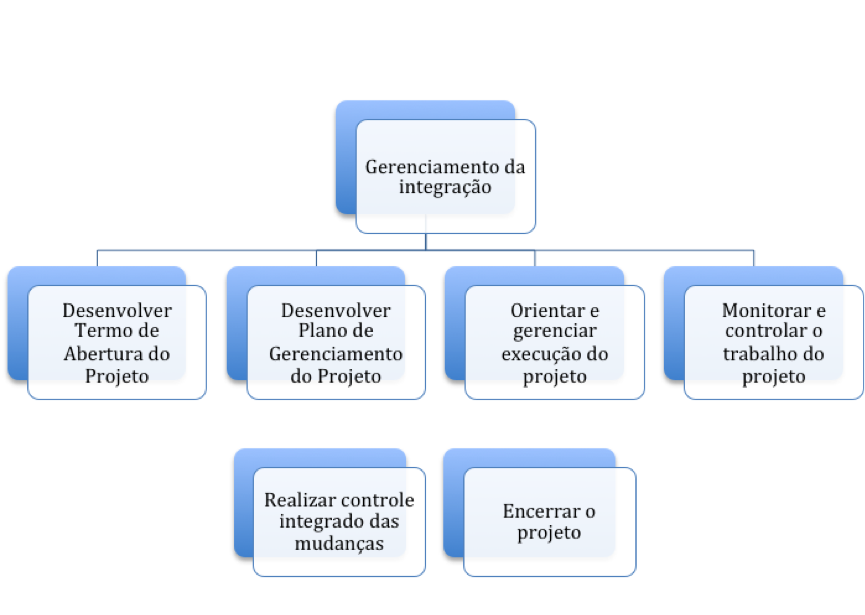
\includegraphics[scale=0.75]{Figuras/gerenciamento_integracao.png}
\caption{Processos do Gerenciamento da Integração}
\label{fig:proc:ger:integr}
\end{figure}

\section{\planproj}

O \planproj é um documento usado no auxílio da gerência do projeto no seu dia a dia. Ele é formalizado e aprovado pelos \stake e deve conter informações realistas sobre o projeto.

Ele é composto por:

\begin{itemize}

\item Plano do planejamento

\item Planos de gerenciamento de todas as áreas que serão controladas

\item Linha de base do escopo, cronograma e orçamento

\item Outros documentos e processos importantes para o gerenciamento do projeto

\end{itemize}

\subsection{Plano do planejamento}

É considerado como o pré-planejamento. Consiste em atribuir datas, responsáveis e tarefas com o objetivo de planejar o projeto e gerar os documentos e informações necessárias para a \kick. A Figura \ref{fig:plano:planejamento} mostra um exemplo de plano contendo algumas das tarefas mais importantes.

\begin{figure}[!h]
\centering
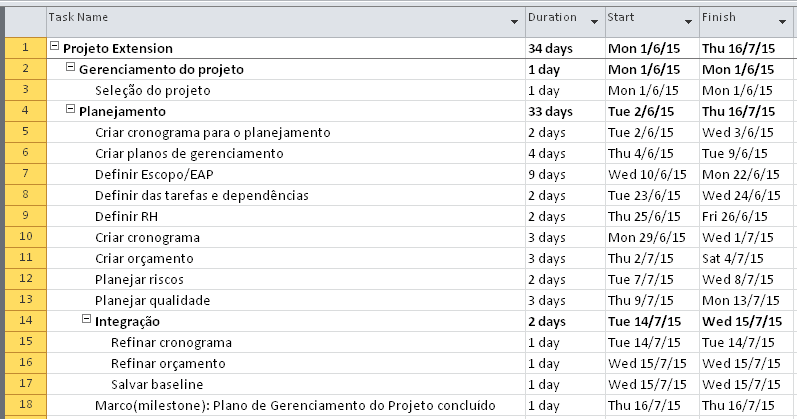
\includegraphics[scale=0.5]{Figuras/plano_planejamento.png}
\caption{Exemplo de Plano do Planejamento}
\label{fig:plano:planejamento}
\end{figure}

\subsection{\Kick}

É o evento que formaliza o início do projeto e que tem como um dos objetivos principais deixar claro os papéis e responsabilidades de todos no projeto. Por isso a participação de todos os \stake é de suma importância. Trata-se de uma ótima oportunidade de colocar frente a frente a equipe, clientes e outros \stake.

\subsection{Integracão dos planos}

Um projeto é como um organismo vivo no qual uma deficiência em uma área pode influenciar uma ou mais outras áreas. Quanto mais tarde essa deficiência for detectada e corrigida, piores serão as consequências.

Por este motivo, os planos de gerenciamento das diversas áreas do projeto não podem ser considerados totalmente independentes e devem ser construídos e mantidos de forma integrada.

Os planos de gerenciamento do projeto seguem as áreas de conhecimento que serão estudadas:

\begin{itemize}

\item \planesc
\item \plancron
\item \plancusto
\item \planqual
\item \planpess
\item \plancom
\item \planrisco
\item \planaq

\end{itemize}

Organizações que possuem escritórios de projeto (PMO) podem definir planos de gerenciamentos padronizados para que não se perca tempo com processos que se repetem em cada novo projeto. Neste caso, cabe ao \gp seguir os processos e planos definidos e o Plano do Planejamento vai incluir somente o cronograma das etapas.

\subsection{Processo Desenvolver o \planproj}

\begin{figure}[!h]
\centering
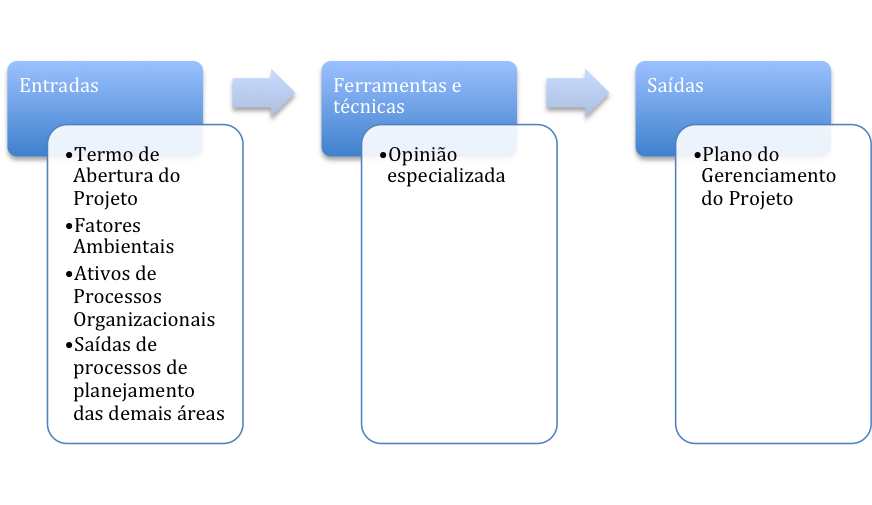
\includegraphics[scale=0.75]{Figuras/proc_integracao_1.png}
\caption{Processo Desenevolver o \planproj}
\label{fig:proc:des:planproj}
\end{figure}

\subsubsection{Entradas}

\begin{itemize}

\item \termo: principal base para início do planejamento, pois possui tudo que ja foi definido para o projeto até o momento.

\item \amb: cultura, infraestrutura, mercado, normas, etc.

\item \ativ: processos e métodos pré-definidos, informações históricas, lições aprendidas, etc.

\item Saidas de processos de planejamento das demais áreas: geram documentos e informações que devem ser integradas para a criação do \planproj. Alterações nestes planos geram alterações no \planproj.

\end{itemize}

\subsubsection{Ferramentas e técnicas}

Opinião especializada:

\begin{itemize}

\item Entender as necessidades do projeto e customizar os processos de acordo

\item Desenvolver e incluir no \planproj detalhes de nível técnico ou gerencial

\item Determinar recursos e conhecimentos necessários para execução do \planproj.

\item Identificar quais documentos necessitam de um processo formal de controle de mudanças.

\end{itemize}

\subsubsection{Saídas}

\planproj.

\subsection{Conteúdo do \planproj}

Além dos demais planos de gerenciamento, o \planproj deve definir:

\begin{itemize}

\item Controle de criação de documentos: quais documentos são necessários, quem tem a responsabilidade de criá-los e quando.

\item Planos auxiliares para gerenciamento das áreas de conhecimento.

\item Linhas de base do escopo, tempo e custo e a formalização dos processos de mudança dessas linhas de base.

\item Processo de controle de mudança:

	\begin{itemize}

	\item Pessoas autorizadas a requisitar mudanças.

	\item Processo de solicitação de mudanças.

	\item Fluxo/processo da mudança:

		\begin{itemize}

		\item Recepção
		\item Análise/avaliação
		\item Classificação
		\item Aprovação
		\item Priorização

		\end{itemize}

\end{itemize}

\end{itemize}


%\bibliographystyle{plain}
%\bibliographystyle{bibstyle/latex8}     
%\bibliographystyle{apalike-url}     


\bibliographystyle{Bibliografia/apalike-pt}     

%\bibliographystyle{lastchecked}     
            
\bibliography{Bibliografia/research}

\end{document}